\documentclass[a4paper,12pt]{article}
\usepackage[utf8]{inputenc}
\usepackage[T1]{fontenc}
\usepackage{lmodern}
\usepackage{geometry}
\usepackage{setspace}
\usepackage{fancyhdr}
\usepackage{hyperref}
\usepackage{amsmath}
\usepackage{amsfonts}
\usepackage{amssymb}
\usepackage{mathtools}
\usepackage{float}
\usepackage{tabularx}
\usepackage{enumitem}
\usepackage{graphicx}
\usepackage{ragged2e}
\usepackage[spanish]{babel}
\usepackage{booktabs}
\usepackage{longtable}
\usepackage{multirow}
\usepackage{xcolor}
\usepackage{microtype}
\usepackage{caption}
\usepackage{textcomp}
\newcommand{\euro}{\texteuro}
\newcommand{\E}{\mathbb{E}}
\newcommand{\Var}{\mathrm{Var}}
\newcommand{\Cov}{\mathrm{Cov}}
\newcommand{\VaR}{\mathrm{VaR}}
\newcommand{\TVaR}{\mathrm{TVaR}}
\addto\captionsspanish{\renewcommand{\tablename}{Tabla}}
\addto\captionsspanish{\renewcommand{\figurename}{Figura}}
\captionsetup{font=small,labelfont=bf}

% Configuración de márgenes
\geometry{left=2.5cm,right=2.5cm,top=3cm,bottom=3cm}

% Configuración de encabezados y pies de página
\pagestyle{fancy}
\fancyhf{}
\renewcommand{\headrulewidth}{0pt}
\fancyfoot[C]{\thepage}

% Configuración de interlineado
\onehalfspacing
\justifying

% Configuración de hipervínculos
\hypersetup{
    hidelinks,
    colorlinks=false
}

\begin{document}

% Primera página (Título, Resumen y Abstract)
\begin{titlepage}
    \centering
    \vspace*{0.1cm}
    \huge\textbf{Tema 2: Preguntas de debate}\\
    \vspace{1cm}
    \small{Luiz Alberto Luzuriaga Izquierdo}\\
    \vspace{0.1cm}
    Facultad de ciencias económicas, empresariales y turismo. \\
    \vspace{0.1cm}
    Universidad de Alcalá de Henares. \\
    \vspace{0.1cm}
    Curso 2026-2027\\
    \vspace{0.5cm}

{\bfseries Resumen}

\vspace{0.1cm}
\noindent
\begin{justify}
Respuestas argumentadas a las preguntas de debate del tema, con cifras de los casos prácticos. Tema 2 (Modelo individual del coste total de siniestralidad): Suma de riesgos independientes póliza a póliza, aproximaciones de tres momentos y comparación con la distribución exacta.\\\\
\vspace{0.1cm}
\noindent
\textbf{Palabras clave}: modelo individual, Normal Power, Gamma trasladada, preguntas de debate.
\end{justify}
\begin{center}
    {\bfseries Abstract}
\end{center}
\vspace{0.1cm}
\noindent
\begin{justify}
Class work for Topic 2 of Actuarial Mathematics of Stability and Solvency of Insurance Activity: discussion questions with actuarial reasoning and numerical evidence.\\\\
\vspace{0.1cm}
\noindent
\textbf{Keywords}: individual risk model, Normal Power, shifted Gamma, discussion questions.
\end{justify}

\end{titlepage}

% Índice
\newpage\pagenumbering{gobble}
\renewcommand{\contentsname}{Índice}
\newgeometry{left=4cm, right=4cm, top=3cm, bottom=2.5cm}
\tableofcontents

\restoregeometry
\newpage
\numberwithin{equation}{section}
\pagenumbering{arabic}
\setcounter{page}{1}

\section{Tema 2: Modelo individual del coste total de siniestralidad}
\label{sec:tema2debate}
\noindent
Respuestas argumentadas a las preguntas de debate del tema, con cifras de los casos prácticos. Material de referencia: diapositivas del Tema 2 (Prof. Hugo González Riera).

\subsection{Debate 1 -- Pandemia o cat\'astrofe que correlaciona las $X_i$}

\paragraph{Tesis.} El modelo individual deja de ser v\'alido, y lo hace de la peor manera posible: sigue dando un n\'umero, pero ese n\'umero ya no mide el riesgo. La independencia es la hip\'otesis que sostiene la diversificaci\'on.

\paragraph{1. Qu\'e se rompe.} Con independencia, $\Var(S)=\sum\Var(X_i)$ crece como $n$ y la desviaci\'on relativa $SD/\E[S]$ decrece como $1/\sqrt n$. Con un shock com\'un, aparecen $n(n-1)$ covarianzas y la desviaci\'on relativa se estabiliza en un valor positivo que \emph{no se diversifica}. La TCL tampoco se aplica: la distribuci\'on agregada tiene la cola de la mezcla y no la de la Normal.

\paragraph{2. Dos formas de verlo.}
\begin{itemize}[leftmargin=*,itemsep=1pt]
\item \textbf{Correlaci\'on constante $\rho$.} $\Var(S)=(1-\rho)\sum\Var(X_i)+\rho\big(\sum SD(X_i)\big)^2$. En el Caso~1, $\rho=0{,}001$ multiplica la varianza por $1{,}67$ y el VaR Normal pasa de $1.491.844$ a $1.750.382$ \euro; con $\rho=0{,}005$ la varianza se multiplica por $4{,}4$ y el VaR llega a $2.451.674$ \euro.
\item \textbf{Factor com\'un de mortalidad (mezcla).} Se supone que las probabilidades son $\Theta q_i$ con $\E[\Theta]=1$ y $\mathrm{sd}(\Theta)=\tau$ (por ejemplo, un a\~no de gripe o pandemia que multiplica la mortalidad). Entonces $\Var(S)=\E[\Var(S\mid\Theta)]+\Var(\E[S\mid\Theta])\approx\Var_{\text{ind}}+\tau^2\E[S]^2$. Con $\tau=0{,}3$: varianza $\times1{,}29$ y VaR Normal $1.609.923$ (+7,9\,\%); con $\tau=0{,}5$: varianza $\times1{,}79$ y VaR $1.791.042$ (+20\,\%). Adem\'as aumenta la asimetr\'ia, de modo que la Normal infravalora todav\'ia m\'as.
\end{itemize}
\begin{figure}[H]\centering
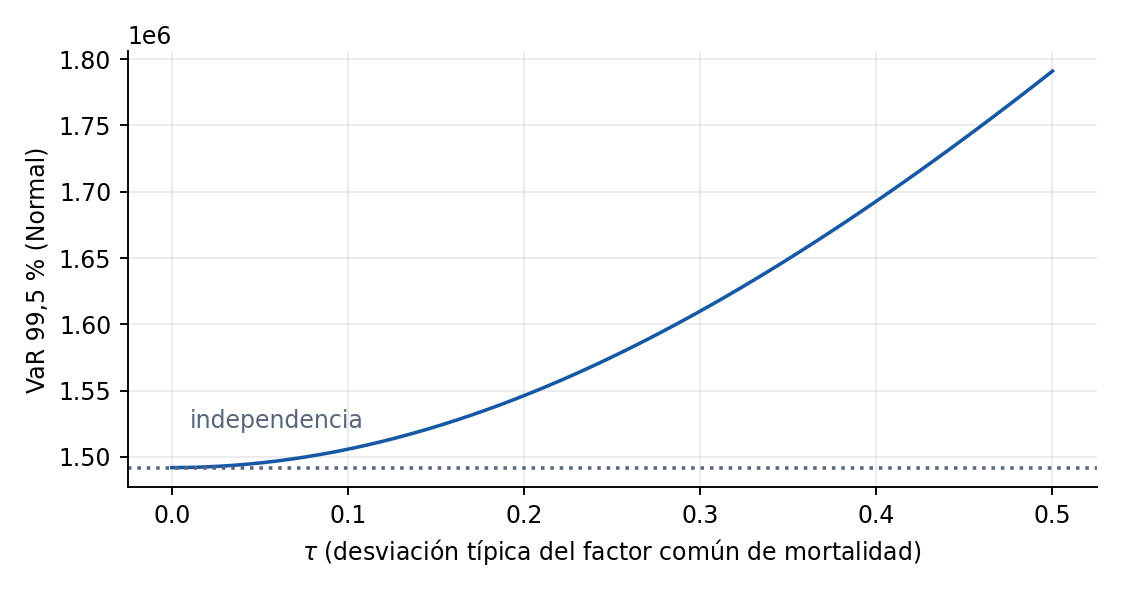
\includegraphics[width=.72\linewidth]{t2_f_debate1.png}
\caption{VaR 99,5\,\% (Normal) del Caso~1 al introducir un factor com\'un de mortalidad de desviaci\'on $\tau$.}
\end{figure}

\paragraph{3. La diversificaci\'on mata el riesgo idiosincr\'asico, no el sist\'emico.} Si se multiplica la cartera por $1.000$ (un millón de p\'olizas), el capital por independencia sube solo como $\sqrt{1000}$: $2{,}576\cdot10{,}83\text{ M}=27{,}9$ M\euro, un $4{,}6\%$ de $\E[S]=610$ M\euro. En cambio, el submódulo de cat\'astrofe de mortalidad de la f\'ormula est\'andar de Solvencia~II (aumento de $0{,}15$ puntos porcentuales en las tasas de mortalidad durante 12 meses) crece proporcionalmente con la cartera: $0{,}0015\cdot1{,}4\cdot10^{11}=210$ M\euro. El riesgo sist\'emico es $7{,}5$ veces el capital que da el modelo individual. Con 1.000 p\'olizas ocurre lo contrario ($210.000$ frente a $881.844$), que es la raz\'on de que el modelo parezca razonable en el aula y no en una aseguradora grande.

\paragraph{4. Qu\'e hacer.}
\begin{itemize}[leftmargin=*,itemsep=1pt]
\item Incorporar el factor com\'un expl\'icitamente (modelo de mezcla Poisson--Gamma, Binomial Negativa, escenarios) o \emph{sumar} un m\'odulo de cat\'astrofe al capital idiosincr\'asico con una matriz de correlaci\'on, como hace la f\'ormula est\'andar.
\item Trasladar el riesgo: reaseguro cat\'astrofe (exceso de p\'erdida por evento, \emph{stop-loss} agregado) o titulizaci\'on (bonos de mortalidad).
\item Documentar y validar la hip\'otesis de independencia en los modelos internos: la propia normativa lo exige.
\end{itemize}

\bigskip\hrule\bigskip

\subsection{Debate 2 -- Capital si sustituimos el modelo individual por el colectivo}

\paragraph{Tesis.} Con la misma cartera, el cambio de modelo en s\'i apenas mueve el capital cuando las probabilidades son peque\~nas; lo que lo mueve de verdad son los supuestos adicionales que permite el colectivo (varios siniestros por p\'oliza, sobredispersi\'on, severidad no acotada).

\paragraph{1. Qu\'e cambia matem\'aticamente.} El colectivo representa $S=\sum_{j=1}^NY_j$ con $N\sim\text{Poisson}(\lambda)$, $\lambda=\sum q_i$ y una severidad mezcla. Mismas medias: $\E[S]=\sum q_i\mu_i$. Las varianzas difieren:
\[
\Var_{\text{col}}(S)-\Var_{\text{ind}}(S)=\sum_i q_i^2\mu_i^2\ \ge0 ,
\]
porque el colectivo permite m\'as de un siniestro por p\'oliza y no impone $\Var(I_i)=q_i(1-q_i)$ sino $q_i$ (Poisson frente a Bernoulli). Lo mismo ocurre con el tercer momento: $\sum q_ib_i^3$ frente a $\sum q_i(1-q_i)(1-2q_i)b_i^3$.

\paragraph{2. Cifras.}
\begin{center}
\begin{tabular}{lrrrr}
\toprule
Cartera & $\Var_{\text{ind}}$ & $\Var_{\text{col}}$ & $\Delta$ varianza & $\Delta$ VaR Normal\\
\midrule
Caso 1 (Vida, $q\le0{,}01$) & $1{,}172\cdot10^{11}$ & $1{,}180\cdot10^{11}$ & $+0{,}68\%$ & $+0{,}20\%$\\
8 p\'olizas del taller & $1{,}310\cdot10^{9}$ & $1{,}318\cdot10^{9}$ & $+0{,}63\%$ & --\\
Caso 2 (Accidentes, $q$ 5--8\,\%) & $4{,}651\cdot10^{8}$ & $4{,}897\cdot10^{8}$ & $+5{,}29\%$ & $+1{,}04\%$\\
\bottomrule
\end{tabular}
\end{center}
El Poisson compuesto es \emph{conservador} y la diferencia es del orden de $q$: despreciable en Vida con $q\le1\%$, apreciable en accidentes o salud con $q\approx5$--$10\%$.

\paragraph{3. Lo que s\'i cambia el capital: la sobredispersi\'on.} Si el n\'umero de siniestros no es Poisson sino Binomial Negativa con $\Var(N)=\phi\lambda$, entonces $\Var(S)=\lambda\E[B^2]+(\phi-1)\lambda\,\E[B]^2$. En el Caso~1 ($\lambda=3{,}6$, $\E[B]=169.444$):
\begin{center}
\begin{tabular}{lrrr}
\toprule
$\phi=\Var(N)/\lambda$ & $SD(S)$ & VaR 99,5\,\% Normal & vs Poisson\\
\midrule
1 (Poisson) & 343.511 & 1.494.826 & --\\
1,5 & 411.923 & 1.671.043 & $+12{,}0\%$\\
2 & 470.490 & 1.821.903 & $+22{,}1\%$\\
\bottomrule
\end{tabular}
\end{center}
Una dispersi\'on moderada del n\'umero de siniestros (que representa incertidumbre de par\'ametro o heterogeneidad no observada) pesa m\'as que todo el cambio individual$\to$colectivo.

\paragraph{4. Otras consecuencias.}
\begin{itemize}[leftmargin=*,itemsep=1pt]
\item \textbf{C\'alculo}: el colectivo (clase $(a,b,0)$) admite la recursi\'on de Panjer y FFT; el individual necesita convoluci\'on o De Pril. Con muchas p\'olizas el colectivo es mucho m\'as \'agil.
\item \textbf{Informaci\'on}: el individual conserva la heterogeneidad y permite decisiones por p\'oliza; el colectivo la promedia. Si la cartera cambia de composici\'on el colectivo se queda atr\'as.
\item \textbf{Aproximaciones}: la asimetr\'ia del colectivo es algo mayor (m\'as cola), as\'i que la brecha Normal/exacto no desaparece.
\end{itemize}

\paragraph{Conclusi\'on.} Cambiar de individual a colectivo sube el capital en torno a $q$ (0,2--1\,\% aqu\'i); los supuestos de frecuencia (sobredispersi\'on) pueden subirlo un 10--20\,\%. La elecci\'on debe hacerse por la informaci\'on disponible y el uso, no por el capital.

\bigskip\hrule\bigskip

\subsection{Debate 3 -- Reaseguro, asimetr\'ia y fiabilidad de las aproximaciones}

\paragraph{Tesis.} La pregunta sugiere que el reaseguro reduce la asimetr\'ia y que por eso las aproximaciones son m\'as fiables. Es cierto solo en parte, y los n\'umeros muestran un matiz importante: el reaseguro \emph{proporcional} no cambia $\gamma_S$, y el de \emph{exceso por riesgo} la reduce poco porque la asimetr\'ia de esta cartera viene de la baja frecuencia.

\paragraph{1. Qu\'e hace cada tipo de reaseguro.}
\begin{itemize}[leftmargin=*,itemsep=1pt]
\item \textbf{Cuota-parte (retenci\'on $c$).} $S_{\text{ret}}=cS$: media $c\E[S]$, desviaci\'on $c\,SD$, y asimetr\'ia $\gamma_S$ \emph{sin cambios}. Con $c=0{,}5$: $SD=171.177$, $\gamma=0{,}627$. Reduce el capital, pero la Normal infravalora lo mismo, en proporci\'on.
\item \textbf{Exceso de p\'erdida por riesgo (retenci\'on $d$).} Cada cuant\'ia queda limitada a $\min(b_i,d)$. Recorta la severidad m\'axima (cuyo efecto en el tercer momento es c\'ubico) y por tanto reduce la dispersi\'on de capitales.
\item \textbf{Stop-loss agregado.} Trunca la cola de $S$ en $M$: la asimetr\'ia de la parte retenida baja de forma dr\'astica.
\end{itemize}

\paragraph{2. Datos del Caso 1 con exceso de p\'erdida por riesgo.}
\begin{center}
\begin{tabular}{rrrrrrr}
\toprule
Retenci\'on $d$ & $\E[S]$ & $SD$ & $\gamma_S$ & VaR Normal & VaR exacto & Error Normal\\
\midrule
sin reaseguro & 610.000 & 342.354 & 0,627 & 1.491.844 & 1.700.000 & $-12{,}2\%$\\
250.000 & 585.000 & 321.859 & 0,589 & 1.414.055 & 1.600.000 & $-11{,}6\%$\\
200.000 & 560.000 & 304.066 & 0,567 & 1.343.222 & 1.500.000 & $-10{,}5\%$\\
150.000 & 490.000 & 261.033 & 0,541 & 1.162.375 & 1.300.000 & $-10{,}6\%$\\
100.000 & 360.000 & 189.283 & 0,523 & 847.560 & 900.000 & $-5{,}8\%$\\
\bottomrule
\end{tabular}
\end{center}
El exceso por riesgo reduce el capital (de $1,09$ a $0,54$ M\euro\ de capital sobre la media) pero la asimetr\'ia solo baja de $0{,}63$ a $0{,}52$ y el error de la Normal sigue siendo del $6$--$12\%$.

\paragraph{3. Por qu\'e la asimetr\'ia no se va.} Si todas las cuant\'ias fueran iguales a $b$, $S=b\,N$ con $N$ casi Poisson de media $\lambda=\sum q_in_i=3{,}6$, y la asimetr\'ia es $1/\sqrt\lambda=0{,}527$. Ese es el \emph{suelo}: lo determina la \emph{frecuencia esperada} de siniestros, no el reaseguro. Los 3,6 fallecimientos esperados al a\~no no bastan para que act\'ue el TCL. Para reducir de verdad la asimetr\'ia habr\'ia que aumentar $\lambda$ (m\'as p\'olizas o carteras agrupadas) o truncar la cola con un stop-loss.

\paragraph{4. Por qu\'e importa para la fiabilidad.} La precisi\'on de una aproximaci\'on de dos momentos depende de $\gamma_S$ y de $z_p$ (el error de la Normal es del orden $\gamma_S(z_p^2-1)/6$ desviaciones t\'ipicas). Las aproximaciones de tres momentos (Normal Power, Gamma trasladada) siguen dando errores por debajo del $1\%$ en todos los niveles de retenci\'on mientras $S$ no sea demasiado discreta (con $d=100.000$, $S$ solo toma valores m\'ultiplos de $100.000$ y el error NP del $+4{,}5\%$ es un efecto de rejilla). La moraleja operativa: reasegurar no sustituye a usar una aproximaci\'on que capture la asimetr\'ia; y la reducci\'on del capital por reaseguro hay que calcularla sobre la distribuci\'on neta con el mismo cuidado.

\paragraph{5. Coste y contrapartida.} Reasegurar tiene un coste (prima de reaseguro $>$ pura) y a\~nade riesgo de contraparte (en Solvencia~II, SCR de incumplimiento de contraparte, aunque el reaseguro se reconoce como t\'ecnica de mitigaci\'on). Lo que se paga es la reducci\'on de $\sigma$, no una mejora de la forma de la distribuci\'on.

\bigskip\hrule\bigskip

\subsection{Debate 4 -- Datos escasos de severidad en capitales elevados}

\paragraph{Tesis.} Aqu\'i el problema no es elegir entre dos f\'ormulas sino repartir el riesgo de modelo: con pocos datos, el individual tiene mucha varianza de estimaci\'on y el colectivo tiene sesgo. Lo habitual es combinarlos.

\paragraph{1. Qu\'e pasa en cada modelo.}
\begin{itemize}[leftmargin=*,itemsep=1pt]
\item \textbf{Individual.} Para cada p\'oliza de capital alto hace falta una severidad propia. En Vida con capital fijo (severidad degenerada $B_i=b_i$) no hay problema: $b_i$ se conoce. En no-vida o accidentes con severidad aleatoria y muy pocas observaciones, la estimaci\'on de $(\mu_i,\sigma_i^2)$ es ruidosa, y el sobreajuste produce tarifas y capitales inestables.
\item \textbf{Colectivo.} Agrupa todas las cuant\'ias en una sola distribuci\'on y toma prestada fuerza estad\'istica; pero esa distribuci\'on est\'a dominada por los siniestros peque\~nos y habituales, y la cola de los capitales altos queda mal representada (sesgo hacia abajo).
\end{itemize}

\paragraph{2. Compromisos (sesgo--varianza).}
\begin{center}
\begin{tabular}{p{3.2cm}p{5.6cm}p{5.6cm}}
\toprule
 & Individual & Colectivo\\
\midrule
Sesgo & bajo (respeta cada p\'oliza) & alto en la cola de capitales altos\\
Varianza de estimaci\'on & alta con pocos datos & baja (agrupa)\\
Trazabilidad & por p\'oliza & global\\
Uso en suscripci\'on & directo & indirecto\\
\bottomrule
\end{tabular}
\end{center}

\paragraph{3. Cu\'anto pesa la incertidumbre de par\'ametros (Caso 1).} Si $q_D$ (el grupo de capital $300.000$) est\'a mal estimada: con $q_D\times1{,}2$ el VaR Normal sube $62.513$ \euro\ (+4,2\,\%) y con $\times1{,}5$ sube $153.990$ \euro\ (+10,3\,\%). Si todas las $q$ est\'an un $20\%$ infravaloradas, el capital sube un $13{,}8\%$. El error de estimaci\'on es del mismo orden que el de la elecci\'on de modelo.

\paragraph{4. Soluciones pr\'acticas.}
\begin{enumerate}[leftmargin=*,itemsep=2pt]
\item \textbf{Modelo h\'ibrido.} Los grandes riesgos identificables (capital por encima de un umbral) se tratan \emph{individualmente}, con $q_i$ y $b_i$ expl\'icitos, o por \emph{juicio experto}; el resto (\emph{attritional}) se agrupa en un colectivo.
\item \textbf{Credibilidad (B\"uhlmann).} Combinar la experiencia propia del segmento con la del mercado o un benchmark: $\hat q=Z\,\bar q_{\text{propia}}+(1-Z)\,q_{\text{mercado}}$, con $Z=n/(n+k)$.
\item \textbf{Teor\'ia de valores extremos.} Para la cola de severidad, ajustar una Pareto generalizada por encima de un umbral (Tema 5) en lugar de una distribuci\'on para todo el rango.
\item \textbf{Enfoque bayesiano / incertidumbre de par\'ametros.} Propagar la incertidumbre en $(q,\mu,\sigma)$ al capital, con distribuciones a priori informadas por el mercado. Es la v\'ia natural del \emph{margen de prudencia}.
\item \textbf{Reaseguro del riesgo de cola.} Un exceso de p\'erdida por riesgo limita el efecto de las severidades mal estimadas.
\end{enumerate}

\paragraph{5. Marco regulatorio.} La Directiva~2009/138/CE (art.~82) exige que los datos usados para las provisiones sean apropiados, completos y exactos, y admite aproximaciones con justificaci\'on proporcional; los modelos internos deben documentar los supuestos y su sensibilidad. Con datos escasos la autoridad espera ver m\'argenes de prudencia y an\'alisis de sensibilidad expl\'icitos.

\paragraph{Conclusi\'on.} Con pocos datos de capitales elevados, el compromiso es entre sesgo (colectivo) y varianza (individual). La respuesta profesional es h\'ibrida: individual para los pocos riesgos grandes que se conocen uno a uno, colectivo con credibilidad para el resto, y cuantificaci\'on expl\'icita de la incertidumbre de par\'ametros.

\subsubsection*{Referencias}
\begin{itemize}[leftmargin=*,itemsep=0pt]
\item Kaas, R., Goovaerts, M., Dhaene, J. y Denuit, M. (2008). \emph{Modern Actuarial Risk Theory} (2.\textordfeminine\ ed.). Springer.
\item Klugman, S. A., Panjer, H. H. y Willmot, G. E. \emph{Loss Models: From Data to Decisions}. Wiley.
\item B\"uhlmann, H. y Gisler, A. (2005). \emph{A Course in Credibility Theory and its Applications}. Springer.
\item Directiva 2009/138/CE (Solvencia~II) y Reglamento Delegado (UE) 2015/35.
\end{itemize}

\end{document}
